\begin{figure}[ht]
  \centering
  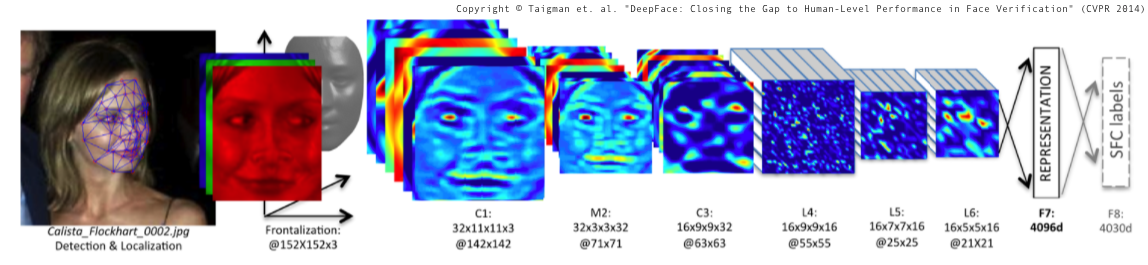
\includegraphics[width=\columnwidth]{deepface-model.png}
  \caption{Facebook DeepFace structure}
  \label{dfstructure}
\end{figure}

\subsection{Facebook DeepFace} \label{sec:deepFace} Due to my lack of experience
in the field of Autoencoders and Deep Learning in general, I decided to use one
of the well known CNNs in the DeepFace community and modify it according to my
chosen dataset.

After some research I have chosen Facebook's facial recognition model
\textit{DeepFace} \cite{taigman2014deepface}. It consists of 9 layers (see Fig.
\ref{dfstructure}), and achieved an accuracy of 97.35\% on the Labeled Faces in
the Wild (LFW) dataset. To turn this classification network into an autoencoder,
one simply needs to mirror the network. However because of hardware constraints
on my personal machine, I will be using pre-trained weights adopted from
\cite{serengil2017tensorflow101}. The author build and trained the renowned
model by scratch using the \textit{VGGFaceset2} dataset. Note that in
\ref{dfstructure} the final layer F8 is dashed. This is because the last softmax
layer is tuned to classify its training set and hence will be dropped for our
feature extraction use case. In our case, only layer F7 will be used to
determine the diagnostic features of each face. As a result, the DeepFace model
turns a 152$\times$152 sized facial image into a 4096 dimensional vector
(embedding), serving as the input attributes to the output classifier. 
